 \section{Fiche de destination}
 \label{sec::sheet_univ}
 
 \begin{figure}[H]
 	\centerline{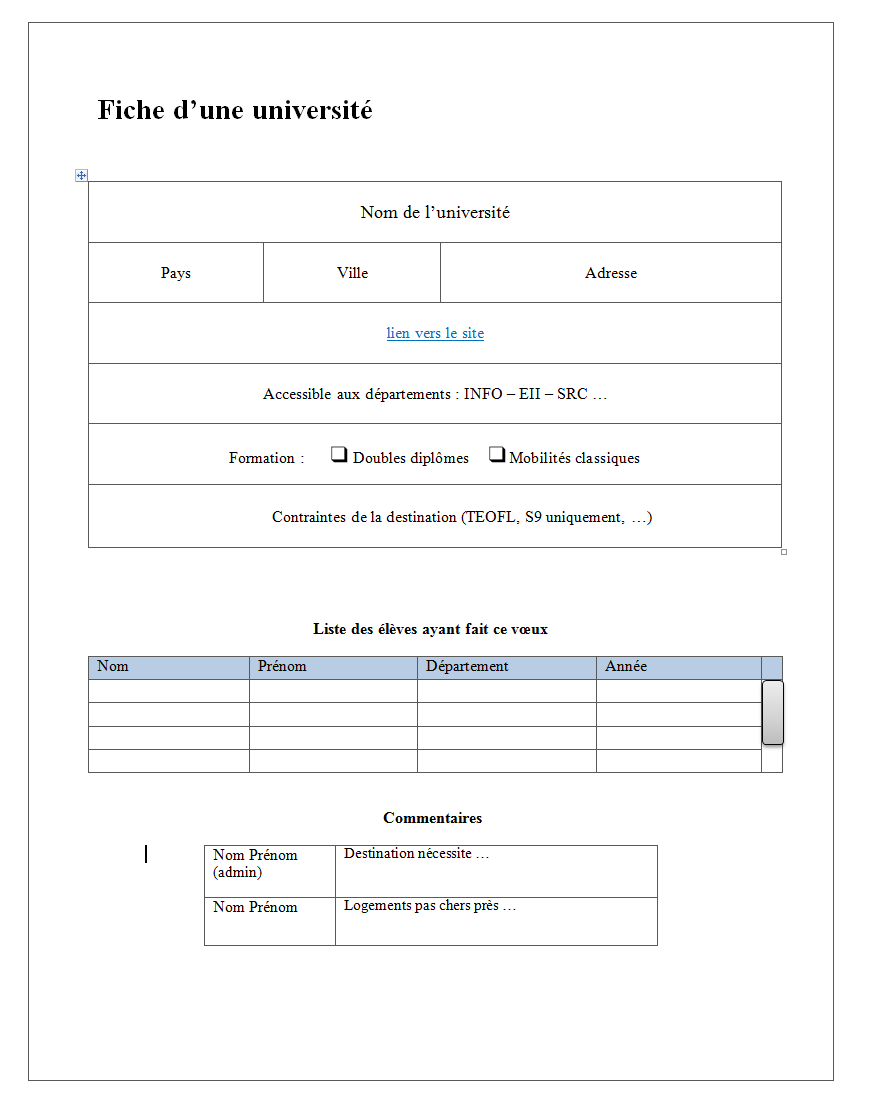
\includegraphics[scale=0.5]{Universites/ficheUniv.png}}
 	\caption{Exemple de fiche descriptive d'un établissement partenaire}
 \end{figure}
 
 Chaque université partenaire disposera d'une fiche où figureront les informations complémentaires au tableau.
 On y trouvera notamment toutes les informations présentes dans le tableau ainsi que :
 \begin{itemize}
 	\item un lien vers le site de l'université ;
 	\item si la destination propose un double diplôme ;
 	\item (facultatifs) certains pré-requis de la destination, comme le TOEFL, ou si la destination n'est disponible qu'en S9 par exemple ;
 	\item les commentaires des responsables RI et des élèves déjà partis sur cette destination ;
 	\item la liste des étudiants ayant déjà choisis ce vœux.
 \end{itemize}
 

 
 Les administrateurs pourront également éditer ou supprimer un partenariat directement depuis la fiche.